\usetikzlibrary{positioning,arrows.meta}
\chapter{Background}
\label{chap:fno}

This chapter provides a comprehensive treatment of the Fourier Neural Operator (FNO)~\cite{li2021fourier}, the primary baseline against which the models developed in this thesis are evaluated. We describe its theoretical foundations in operator learning, its architecture, the benchmark dataset it defines, and its published results on the viscous Burgers equation. Understanding FNO in detail is essential both for interpreting our comparative results and for identifying the structural differences that explain the performance gap between FNO and our TCAN-based approach.

% ===================================================================
\section{Operator Learning: Learning Maps Between Function Spaces}
\label{sec:fno:operator-learning}

Classical supervised machine learning maps finite-dimensional vectors to finite-dimensional vectors: given a fixed-size input $\mathbf{x} \in \mathbb{R}^d$, a neural network learns to produce an output $\mathbf{y} \in \mathbb{R}^m$. For PDE problems, this paradigm is severely limiting. A PDE solution $u : \Omega \times [0,T] \to \mathbb{R}$ is a function, not a vector; and the mapping from initial condition $u_0 \in \mathcal{A}(\Omega)$ to solution $u(\cdot, T) \in \mathcal{U}(\Omega)$ is an \emph{operator} between infinite-dimensional function spaces.

Operator learning, formalised by Kovachki et al.~\cite{kovachki2023neural}, aims to learn such a mapping $\mathcal{G}^\dagger : \mathcal{A} \to \mathcal{U}$ directly from data. The key desideratum is \emph{discretisation-invariance}: the learned operator should produce consistent outputs regardless of the spatial resolution at which the input is discretised and should generalise to resolutions not seen during training. This is impossible for standard neural networks trained on fixed-size grids but is achievable by architectures based on integral transforms, which operate on continuous function representations.

% ===================================================================
\section{FNO Architecture}
\label{sec:fno:architecture}

\subsection{Iterative Operator Approximation}

FNO approximates the solution operator $\mathcal{G}^\dagger$ through a composition of $L$ nonlinear operator layers:
\begin{equation}
  \mathcal{G}^\dagger \approx \mathcal{Q} \circ \sigma(\mathcal{W}_L + \mathcal{K}_L) \circ \cdots \circ \sigma(\mathcal{W}_1 + \mathcal{K}_1) \circ \mathcal{P},
\end{equation}
where $\mathcal{P}$ is a pointwise lifting operator that maps the input function to a higher-dimensional feature space, $\mathcal{Q}$ is a pointwise projection operator that maps back to the output space, and each intermediate layer combines a local linear operator $\mathcal{W}_\ell$ (implemented as a pointwise linear map, i.e.\ a $1\times1$ convolution) with a non-local integral operator $\mathcal{K}_\ell$ (the Fourier layer described below). The nonlinearity $\sigma$ is applied element-wise after each layer.

\subsection{The Fourier Integral Operator Layer}

The core innovation of FNO is the parameterisation of the integral kernel $\mathcal{K}_\ell$ in the Fourier domain. For an input function $v : \Omega \to \mathbb{R}^{d_v}$, the Fourier layer computes:
\begin{equation}
  (\mathcal{K}_\ell\, v)(x) = \mathcal{F}^{-1}\!\left( R_\ell \cdot (\mathcal{F}\, v) \right)(x),
\end{equation}
where $\mathcal{F}$ denotes the (discrete) Fourier transform, $\mathcal{F}^{-1}$ its inverse, and $R_\ell \in \mathbb{C}^{k_{\max} \times d_v \times d_v}$ is a complex-valued weight tensor acting on the truncated set of the $k_{\max}$ lowest Fourier modes. The truncation to $k_{\max}$ modes acts as a low-pass filter that discards high-frequency components of the input, retaining the dominant spatial structure. The full layer update is:
\begin{equation}
  v_{\ell+1}(x) = \sigma\!\left( W_\ell\, v_\ell(x) + \mathcal{F}^{-1}\!\left( R_\ell \cdot \mathcal{F}(v_\ell) \right)(x) \right),
\label{eq:fno-layer}
\end{equation}
where $W_\ell \in \mathbb{R}^{d_v \times d_v}$ is the weight matrix of the local bypass, applied pointwise. Figure~\ref{fig:fno-layer} illustrates the structure of a single Fourier layer.

\begin{figure}[h!]
\centering
\scalebox{0.72}{
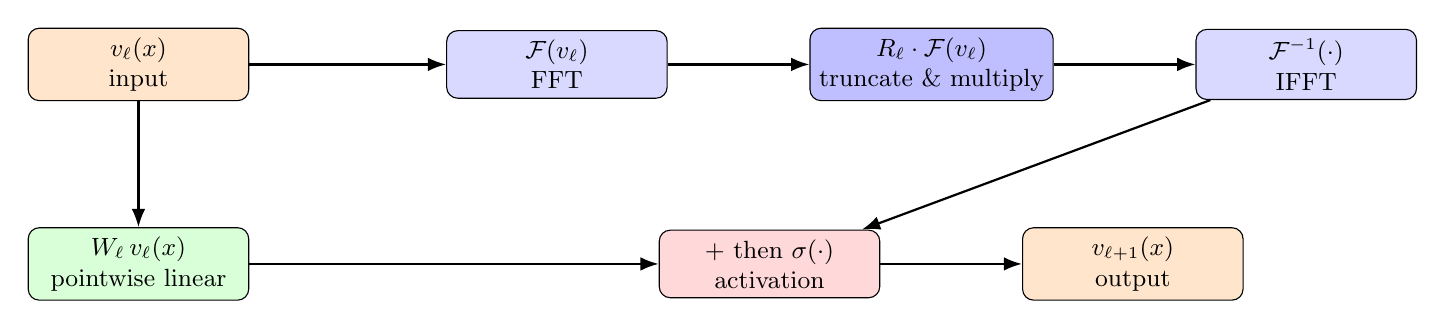
\begin{tikzpicture}[
  box/.style={draw, rounded corners, minimum width=2.8cm, minimum height=0.85cm,
              align=center, font=\small},
  arr/.style={-Latex, thick},
  node distance=1.1cm and 1.8cm
]
  \node[box, fill=orange!20] (v) {$v_\ell(x)$\\input};
  \node[box, fill=blue!15, right=2.5cm of v] (fft)  {$\mathcal{F}(v_\ell)$\\FFT};
  \node[box, fill=blue!25, right=1.8cm of fft] (trunc) {$R_\ell \cdot \mathcal{F}(v_\ell)$\\truncate \& multiply};
  \node[box, fill=blue!15, right=1.8cm of trunc] (ifft) {$\mathcal{F}^{-1}(\cdot)$\\IFFT};
  \node[box, fill=green!15, below=1.6cm of v] (local) {$W_\ell\, v_\ell(x)$\\pointwise linear};
  \node[box, fill=red!15, right=5.2cm of local] (add) {$+$ then $\sigma(\cdot)$\\activation};
  \node[box, fill=orange!20, right=1.8cm of add] (out) {$v_{\ell+1}(x)$\\output};

  \draw[arr] (v) -- (fft);
  \draw[arr] (fft) -- (trunc);
  \draw[arr] (trunc) -- (ifft);
  \draw[arr] (ifft) -- (add);
  \draw[arr] (v) -- (local);
  \draw[arr] (local) -- (add);
  \draw[arr] (add) -- (out);
\end{tikzpicture}
}
\caption{Structure of a single FNO Fourier layer (Equation~\ref{eq:fno-layer}). The global path (top) applies FFT, multiplies the lowest $k_{\max}$ Fourier modes by learnable complex weights $R_\ell$, and maps back with IFFT. The local bypass (bottom) applies a pointwise linear map $W_\ell$. Both paths are summed and passed through a nonlinearity $\sigma$.}
\label{fig:fno-layer}
\end{figure}

\subsection{Discretisation-Invariance}

A key theoretical property of the Fourier layer is that the learned weight tensor $R_\ell$ acts on Fourier coefficients, not on grid points. Because the Fourier transform is resolution-independent (the first $k_{\max}$ modes are the same regardless of the total number of grid points $N \geq 2k_{\max}$), a model trained at one resolution can be evaluated at a different resolution without any architectural change or retraining. In practice, this means a single FNO model trained at $s = 1024$ spatial points can be queried at $s = 64, 128, 256$, or any other resolution, producing consistent predictions. This discretisation-invariance is the central practical advantage of FNO over classical grid-based surrogates and over autoregressive models like TCAN, which must be trained and evaluated at a fixed resolution.

\subsection{Input Encoding and Output Decoding}

For the 1D Burgers problem, the input to FNO is the initial condition $u_0 \in \mathbb{R}^s$ augmented with the spatial coordinate grid $x \in \mathbb{R}^s$, concatenated channel-wise to form a two-channel tensor of shape $(s, 2)$. The lifting operator $\mathcal{P}$ maps this to a $d_v$-channel feature tensor via a pointwise linear layer. After $L = 4$ Fourier layers, the projection operator $\mathcal{Q}$ (a two-layer MLP applied pointwise) maps the $d_v$-channel features to the one-channel output $u(\cdot, T) \in \mathbb{R}^s$.

% ===================================================================
\section{FNO Benchmark Dataset for 1D Burgers}
\label{sec:fno:dataset}

\subsection{Dataset Generation}

The FNO paper defines a standard benchmark dataset for the 1D viscous Burgers equation:
\begin{equation}
  \partial_t u + u\,\partial_x u = \nu\,\partial_{xx} u, \quad x \in [0,1],\; t \in [0,1],
\end{equation}
with periodic boundary conditions and random Gaussian random field initial conditions drawn from $u_0 \sim \mathcal{N}(0, 625(-\Delta + 25I)^{-2})$. Solutions are generated using a split-step pseudo-spectral solver at very high spatial resolution ($s = 8192$ grid points) and then downsampled to the target resolution $s \in \{85, 141, 211, 421\}$ used for training and evaluation. The dataset consists of 1000 training trajectories and 200 test trajectories at each resolution.

This is the \textbf{same dataset} used in our experiments. Switching from our custom dataset to the FNO benchmark allowed us to compare TCAN directly against FNO and all other published baselines that use the same data split.

\subsection{Task Formulation}

The benchmark evaluates models on a \emph{one-shot operator learning} task: given the initial condition $u_0(\cdot)$ at $t=0$, directly predict the solution $u(\cdot, T)$ at a fixed terminal time $T=1$ without intermediate steps. This is a \emph{single forward pass} for FNO. In contrast, our TCAN model operates \emph{autoregressively}: it predicts the solution field at each intermediate time step and rolls out the trajectory step by step, accumulating errors over up to 256 steps to reach $T=1$.

This fundamental difference in task formulation explains a substantial portion of the performance gap between FNO and TCAN: FNO's error is bounded by its one-step approximation quality, whereas TCAN's error grows with the number of rollout steps as small per-step errors compound.

% ===================================================================
\section{FNO Hyperparameters and Training}
\label{sec:fno:training}

For the 1D Burgers benchmark, FNO is trained with the following hyperparameters (as reported in~\cite{li2021fourier}):

\begin{table}[h!]
\centering
\begin{tabular}{ll}
\toprule
\textbf{Hyperparameter} & \textbf{Value} \\
\midrule
Number of Fourier layers ($L$) & 4 \\
Feature channels ($d_v$) & 64 \\
Fourier modes retained ($k_{\max}$) & 16 \\
Activation ($\sigma$) & GeLU \\
Training trajectories & 1000 \\
Batch size & 20 \\
Optimiser & Adam \\
Learning rate & $10^{-3}$ (cosine decay) \\
Epochs & 500 \\
Loss & Relative $L^2$ norm \\
\bottomrule
\end{tabular}
\caption{FNO hyperparameters for the 1D Burgers benchmark~\cite{li2021fourier}.}
\label{tab:fno-hyperparams}
\end{table}

The model is trained to minimise the relative $L^2$ error between the predicted and ground-truth terminal solution:
\begin{equation}
  \mathcal{L}_{\mathrm{FNO}} = \frac{\|\hat{u}(\cdot,T) - u(\cdot,T)\|_{L^2}}{\|u(\cdot,T)\|_{L^2}}.
\end{equation}

% ===================================================================
\section{FNO Results on 1D Burgers}
\label{sec:fno:results}

\subsection{Accuracy and Resolution Scaling}

Table~\ref{tab:fno-results} reports FNO's relative $L^2$ error on the 1D Burgers benchmark across four spatial resolutions. FNO achieves consistently low errors across all resolutions, demonstrating strong discretisation-invariance.

\begin{table}[h!]
\centering
\begin{tabular}{lcccc}
\toprule
\textbf{Method} & $s=85$ & $s=141$ & $s=211$ & $s=421$ \\
\midrule
FNO~\cite{li2021fourier} & 0.0108 & 0.0109 & 0.0109 & 0.0098 \\
\bottomrule
\end{tabular}
\caption{Relative $L^2$ error of FNO on the 1D Burgers benchmark at four spatial resolutions~\cite{li2021fourier}. Lower is better.}
\label{tab:fno-results}
\end{table}

FNO's error remains below $1.1 \times 10^{-2}$ at all resolutions, confirming that the Fourier layer's global receptive field is well-matched to the long-range correlations present in Burgers dynamics. The slight improvement at $s=421$ (from 0.011 to 0.010) suggests that the higher resolution provides a more faithful input representation.

\subsection{Comparison with Other Baselines}

In addition to FNO, the benchmark paper~\cite{li2021fourier} reports results for several other methods on the same dataset:

\begin{table}[h!]
\centering
\begin{tabular}{lcc}
\toprule
\textbf{Method} & \textbf{Rel.\ $L^2$ error} & \textbf{Notes} \\
\midrule
RBM (Reduced Basis)     & $0.0244$ & Linear subspace method \\
FCN (Fully Connected)   & $0.0253$ & Grid-based MLP \\
PCA + NN                & $0.0209$ & PCA compression + MLP \\
LNO (Laplace Neural Op.)& $0.0187$ & Laplace-domain kernel \\
\textbf{FNO}            & $\mathbf{0.0108}$ & Fourier-domain kernel \\
\bottomrule
\end{tabular}
\caption{Comparison of neural PDE surrogates on 1D Burgers at $s=85$~\cite{li2021fourier}. All methods predict $u(\cdot, T=1)$ from $u_0$ in a single forward pass.}
\label{tab:fno-comparison}
\end{table}

FNO outperforms all single-step baselines by a factor of roughly two, confirming that the Fourier parameterisation captures the global structure of the Burgers solution operator more effectively than local or reduced-basis approaches.

\subsection{Computational Efficiency}

Beyond accuracy, FNO offers substantial computational advantages:
\begin{itemize}
  \item \textbf{Speed}: at inference time, FNO applies exactly $L=4$ forward passes of a fixed-size network, regardless of the trajectory length. TCAN requires $T-1$ forward passes for a trajectory of length $T$, making it linearly slower for longer time horizons.
  \item \textbf{Memory}: FNO's memory footprint at inference is dominated by the $k_{\max}$ complex weight tensors $R_\ell$, which are independent of the spatial resolution $s$.
  \item \textbf{No error accumulation}: because FNO maps $u_0 \to u_T$ in a single step, it does not suffer from the autoregressive error accumulation that limits TCAN's accuracy at finer resolutions.
\end{itemize}

% ===================================================================
\section{Why FNO is the Gold Standard Baseline}
\label{sec:fno:baseline}

FNO is the natural baseline for this thesis for three reasons:

\begin{enumerate}
  \item \textbf{Published benchmark}: the FNO paper defines a rigorous benchmark with a fixed dataset, split, and evaluation metric that has been widely adopted. Reporting results on this benchmark makes our work directly comparable to the broader literature.
  \item \textbf{State-of-the-art accuracy}: FNO achieves the lowest relative $L^2$ error among single-step neural operators on the 1D Burgers dataset, establishing a performance ceiling that motivates the analysis of any gap.
  \item \textbf{Architectural contrast}: FNO is a single-step operator learning method with a global spectral receptive field, while our TCAN model is an autoregressive surrogate with local spatial convolutions and temporal attention. Because these two design choices differ along a single axis (one-step versus multi-step rollout), and the performance gap between them is attributable primarily to the formulation, not to the spatial architecture, making the comparison scientifically informative. The quantitative results are reported in Chapter~\ref{chap:approaches}.
\end{enumerate}

The analysis of this gap, and of strategies to close it (progressive rollout training, viscosity conditioning, bounded residual updates), forms the core experimental contribution of Chapter~\ref{chap:approaches}.
